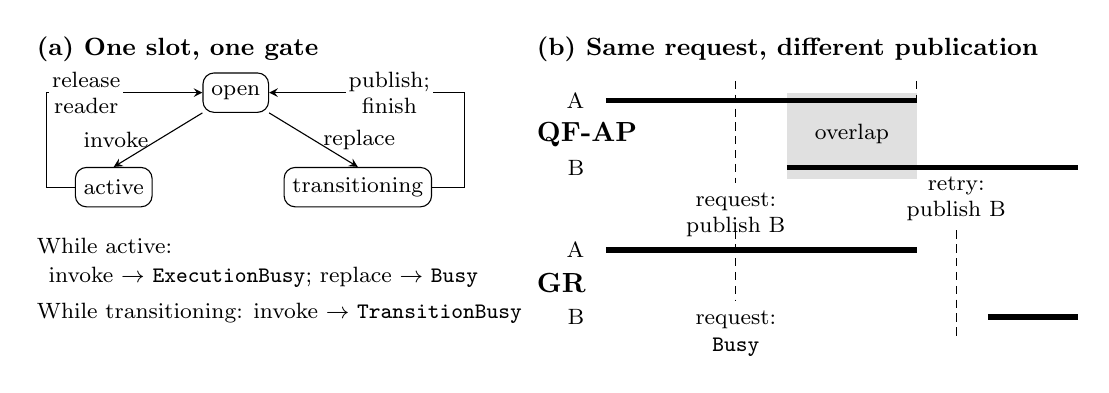
\begin{tikzpicture}[>=stealth, font=\footnotesize,
  state/.style={draw,rounded corners,fill=white,minimum height=5mm,inner sep=3pt},
  live/.style={line width=2pt}, event/.style={densely dashed,thin}]
% One gate: the two downward claims compete for the same open state.
\node[anchor=west,font=\small\bfseries] at (0,3.7) {(a) One slot, one gate};
\node[state] (open) at (2.65,3.15) {open};
\node[state] (active) at (1.1,1.95) {active};
\node[state] (transition) at (4.2,1.95) {transitioning};
\draw[->] (open.south west) -- node[left] {invoke} (active.north);
\draw[->] (open.south east) -- node[right] {replace} (transition.north);
\draw[->] (active.west) -- (.25,1.95) -- (.25,3.15) -- (open.west);
\node[align=center,fill=white,inner sep=1pt] at (.75,3.15) {release\\reader};
\draw[->] (transition.east) -- (5.55,1.95) -- (5.55,3.15) -- (open.east);
\node[align=center,fill=white,inner sep=1pt] at (4.6,3.15) {publish;\\finish};
\node[anchor=west] at (0,1.2) {While active:};
\node[anchor=west] at (.15,.8) {invoke $\to$ \texttt{ExecutionBusy}; replace $\to$ \texttt{Busy}};
\node[anchor=west] at (0,.35) {While transitioning: invoke $\to$ \texttt{TransitionBusy}};

\begin{scope}[xshift=6.35cm]
\node[anchor=west,font=\small\bfseries] at (0,3.7) {(b) Same request, different publication};
% Aligned request and completion times make the two protocols comparable.
\node[anchor=west,font=\bfseries] at (0,2.62) {QF-AP};
\fill[black!12] (3.3,2.05) rectangle (4.95,3.15);
\node at (4.125,2.62) {overlap};
\node[anchor=east] at (.85,3.05) {A};
\node[anchor=east] at (.85,2.2) {B};
\draw[live] (1,3.05) -- (4.95,3.05);
\draw[live] (3.3,2.2) -- (7,2.2);
\draw[event] (2.65,3.3) -- (2.65,2.0);
\node[anchor=north,align=center] at (2.65,2) {request:\\publish B};
\draw[event] (4.95,3.3) -- (4.95,2.95);

\node[anchor=west,font=\bfseries] at (0,.73) {GR};
\node[anchor=east] at (.85,1.15) {A};
\node[anchor=east] at (.85,.3) {B};
\draw[live] (1,1.15) -- (4.95,1.15);
\draw[live] (5.85,.3) -- (7,.3);
\draw[event] (2.65,1.4) -- (2.65,.5);
\node[anchor=north,align=center] at (2.65,.5) {request:\\\texttt{Busy}};
\draw[event] (5.45,1.4) -- (5.45,.05);
\node[anchor=south,align=center] at (5.45,1.4) {retry:\\publish B};
\end{scope}
\end{tikzpicture}
